% \documentclass{article}
% \usepackage{graphicx} % Required for inserting images
% \usepackage{url}
% \usepackage[T2A]{fontenc} % required for russian
% \usepackage{hyphenat}
% \hyphenation{}
% \usepackage[english, russian]{babel}

% \usepackage[a4paper, left=2cm, right=2cm, top=2cm, bottom=2cm]{geometry} % Adjust the margins here

% \usepackage{siunitx} % Required for alignment
% \usepackage{hyperref}
% \geometry{a4paper, margin=1in}

% \title{Поиск сида Minecraft 'Pack.PNG'}
% \author{Наумов Владимир}
% % \date{17 февраля 2025 г.}

% \begin{document}

% \maketitle

% \begin{center}
%     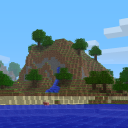
\includegraphics{pack.png}
% \end{center}

% \begin{abstract}
%     Изображение 'Pack.PNG' является культовым символом в сообществе Minecraft, служа дефолтной иконкой для ресурспаков и серверов без пользовательских иконок. Годами происхождение этого изображения, а именно сид мира, из которого оно было сгенерировано в Minecraft, оставалось тайной. Это мини-исследование посвящено результатам его поиска.
% \end{abstract}

% \section{Задача}

% Minecraft использует сиды мира, числовые значения, определяющие процедурную генерацию игровых миров. Каждый сид создает уникальный и консистентный мир, позволяя игрокам делиться и возвращаться к определенным ландшафтам. Сообщество Minecraft@home поставило перед собой цель найти сид, где был сделан снимок 'Pack.PNG'

% \section{Размерности данных}

% Сиды Minecraft являются 48-битными целыми числами, представляющими огромное пространство поиска в $2^{48}$ возможных сидов. Кроме того не была точно известа версия игры на которой был сделан снимок, что усложнило задачу, так как алгоритм генерации мира может отличаться от версии к версии. При том что размеры изображения всего 128x128 пикселей.

% \newpage

% \section{Поиск}

% \subsection{Сид} 
% версия на которой был сделан снимок: development alpha 1.2.2a.
% \subsection{Ориентация}
% была определена по текстурам воды.

% \begin{center}
%     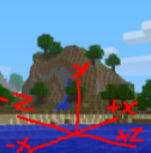
\includegraphics{orientation.png}
% \end{center}

% \subsection{Позиция}
% Целью было определить позицию источника воды, так как он наиболее выделялся.
% Координата Y:

% Уровень моря находится на Y = 64, значит источник находится на Y = 76

% \subsection{Облака}
% Первым прорывом в определении местоположения горы стало обнаружение того, что рисунок облаков один и тот же каждый раз, когда вы запускаете игру. Так же они движутся направлении -X, но не по оси Z. Это позволило определить Z координаты облаков на изображении. 
% Координаты облаков при t = 0:

% \begin{center}
%     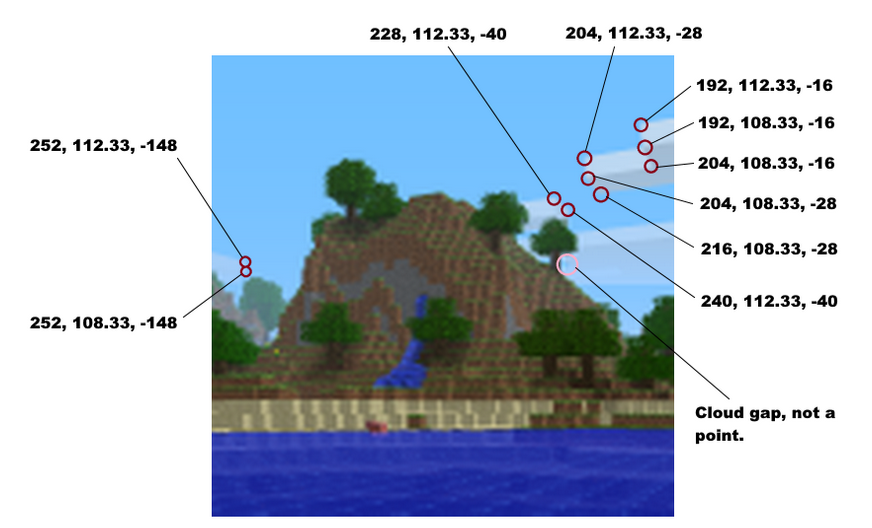
\includegraphics[width=\linewidth]{clouds.png}
% \end{center}

% \subsection{Perspective fitting}

% Определение положения и ориентации игрока можно рассматривать как своего рода задачу регрессии. Воспользовавшись известными трехмерными взаимосвязями, которые видны на изображении, были получены относительно точные оценки.

% Для определения перспективы использовались четыре основных компонента:
% Хорошо виден фасад холма.
% Хорошо видны песчаные глыбы на пляже.
% Облака.
% Текстура воды.
% В процессе оптимизации использовались различные алгоритмы и варьировалось множество различных параметров. Сюда входило не только положение/ориентация игрока, но и любые неизвестные смещения X/Z между различными компонентами. Дополнительно требовалось разрешение экрана и обрезанная часть экрана. Это помогло определить положение игрока относительно облаков и положение холма относительно игрока. В совокупности они дали положение водопада относительно облаков, что позволило определить координату водопада по оси Z.

% \begin{center}
%     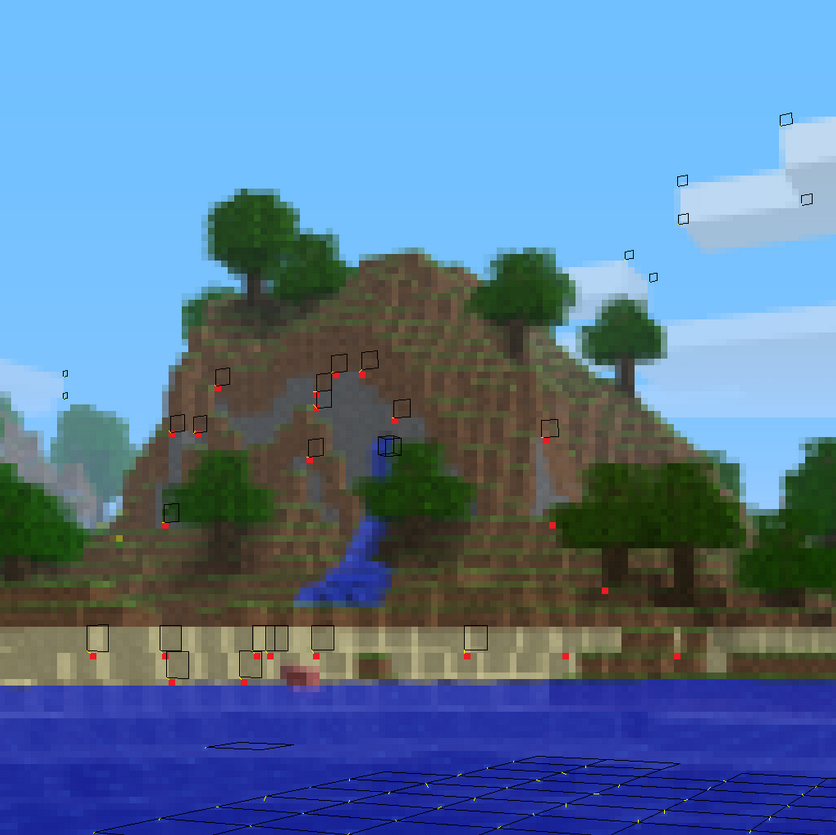
\includegraphics[width=\linewidth]{pfold.png}
% \end{center}

% Были получены оценки, которые позже были улучшены с помощью большего числа точек с изображия.
% Итоговыми оценками стали:
% После небольшого визуального изменения параметров был найден окончательный, очень точный набор координат:
% \begin{enumerate}
%     \item Игрок смещен относительно водопада на (x = -66,84, y = -10,38, z = 31,72).
%     \item Тангаж -8,297, рыскание -119,23.
%     \item Глобальная координата z: z = -31 (в зависимости от положения облака).
%     \item Разрешение экрана — 1600x1116, исходное кадрирование начинается с пикселя (622 284) (полное кадрирование — 512x512).
% \end{enumerate}

% Это было очень важное событие, поскольку оно дало координату Z водопада.

% \subsection{Статистический подход}

% Толщина земли в каждой точке определяется шумом Перлина, который зависит от сида в, в комбинации со случайными "аномалиями" которые одинаковы для всех сидов.
% Исользуя статистические методы(не удалось найти точное описание) была получена координата X = 116.

% Таким образом были получены точные координаты (116, 76, -31)

% \subsection{Поиск сида}

% Был написан алгоритм на Cuda который по патернам земли и песка отбрасывал большиство сидов. Для распределения перебора всех $2^{48}$ уникальных сидов была использована платформа BOINC. 
% Спустя месяцы поиска алгоритм отсеял все сиды кроме 700'000 совпадающих по патернам. Для их проверки был использован более точный алгоритм который обнаружил следующий сид: 3257840388504953787

% \subsection{Результаты}

% Весь процесс поиска занял порядка 8 месяцев и задействовал порядка 3 тысяч человек для брутфорса всех возможных сидов.\\
% В конечном итоге был найден сид на котором был сделан снимок: 3257840388504953787

% \begin{center}
%     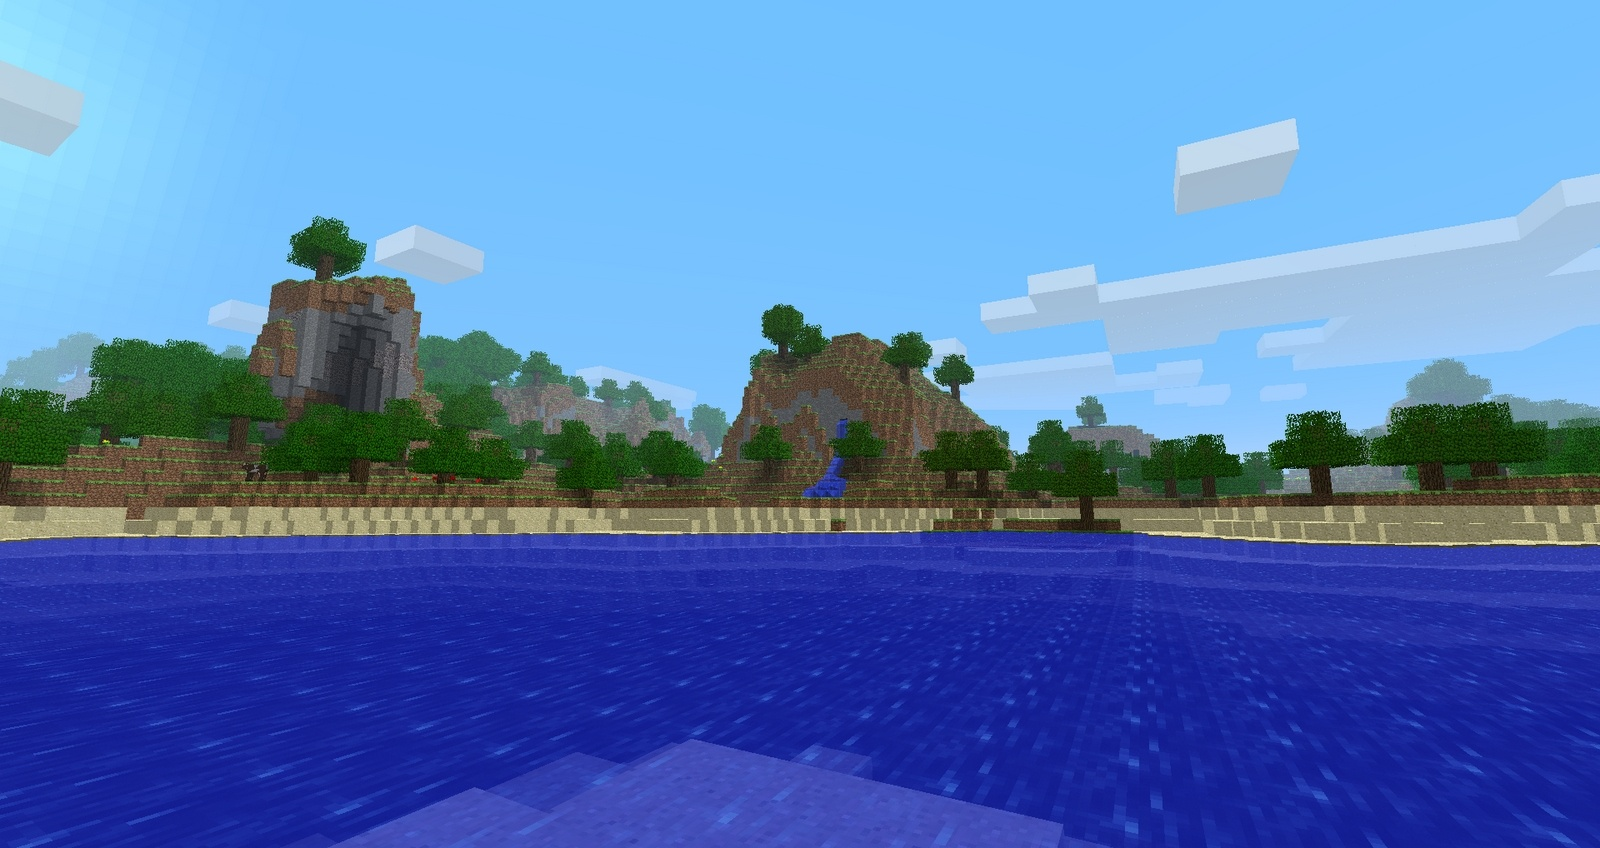
\includegraphics[width=\linewidth]{final.png}
% \end{center}

% % \subsection{Воссоздание ландшафта}

% % Было предринято как минимум 2 крупные попытки воссоздания. Между этими двумя попытками



% \end{document}
\documentclass{article}
\usepackage{graphicx} % Required for inserting images
\usepackage{url}
\usepackage[T2A]{fontenc} % required for russian
\usepackage{hyphenat}
\hyphenation{}
\usepackage[english, russian]{babel}

\usepackage[a4paper, left=2cm, right=2cm, top=2cm, bottom=2cm]{geometry} % Adjust the margins here

\usepackage{siunitx} % Required for alignment
\usepackage{hyperref}
\geometry{a4paper, margin=1in}

\title{Поиск сида Minecraft 'Pack.PNG'}
\author{Наумов Владимир}
% \date{17 февраля 2025 г.}

\begin{document}

\maketitle

\begin{center}
    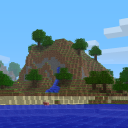
\includegraphics[width=0.5\linewidth]{pack.png} % Adjusted image size
\end{center}

\begin{abstract}
    Изображение 'Pack.PNG' является культовым символом в сообществе Minecraft, служа дефолтной иконкой для ресурспаков и серверов без пользовательских иконок. Годами происхождение этого изображения, а именно сид мира, из которого оно было сгенерировано в Minecraft, оставалось тайной. Это мини-исследование посвящено результатам его поиска. 
\end{abstract}

\section{Задача}

Minecraft использует сиды мира, числовые значения, определяющие процедурную генерацию игровых миров. Каждый сид создает уникальный и консистентный мир, позволяя игрокам делиться и возвращаться к определенным ландшафтам. Сообщество Minecraft@home поставило перед собой цель найти сид, где был сделан снимок 'Pack.PNG'.  

\section{Размерности данных}

Сиды Minecraft являются 48-битными целыми числами, представляющими огромное пространство поиска в $2^{48}$ возможных сидов. Кроме того, не была точно известна версия игры, на которой был сделан снимок, что усложнило задачу, так как алгоритм генерации мира может отличаться от версии к версии. При том, что размеры изображения всего 128x128 пикселей.  

\newpage

\section{Поиск}

\subsection{Сид}
Версия, на которой был сделан снимок: development alpha 1.2.2a.
\subsection{Ориентация}
Была определена по текстурам воды.

\begin{center}
    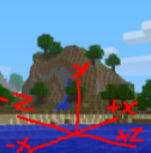
\includegraphics[width=0.5\linewidth]{orientation.png}
\end{center}

\subsection{Позиция}
Целью было определить позицию источника воды, так как он наиболее выделялся.

\textbf{Координата Y:} % Added bold for clarity

Уровень моря находится на Y = 64, значит источник находится на Y = 76.

\subsection{Облака}
Первым прорывом в определении местоположения горы стало обнаружение того, что рисунок облаков один и тот же каждый раз, когда вы запускаете игру. Так же они движутся в направлении -X, но не по оси Z. Это позволило определить Z координаты облаков на изображении.  
Координаты облаков при t = 0:

\begin{center}
    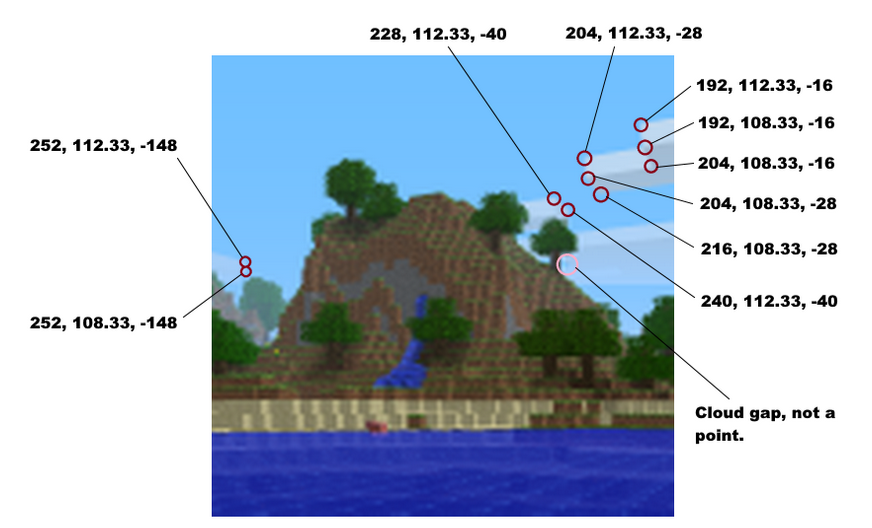
\includegraphics[width=\linewidth]{clouds.png}
\end{center}

\subsection{Perspective fitting}

Определение положения и ориентации игрока можно рассматривать как своего рода задачу регрессии. Воспользовавшись известными трехмерными взаимосвязями, которые видны на изображении, были получены относительно точные оценки.

Для определения перспективы использовались четыре основных компонента:
\begin{itemize} % Changed to itemize for better formatting
    \item Хорошо виден фасад холма.
    \item Хорошо видны песчаные глыбы на пляже.
    \item Облака.
    \item Текстура воды.
\end{itemize}
В процессе оптимизации использовались различные алгоритмы и варьировалось множество различных параметров. Сюда входило не только положение/ориентация игрока, но и любые неизвестные смещения X/Z между различными компонентами. Дополнительно требовалось разрешение экрана и обрезанная часть экрана. Это помогло определить положение игрока относительно облаков и положение холма относительно игрока. В совокупности они дали положение водопада относительно облаков, что позволило определить координату водопада по оси Z.  

\begin{center}
    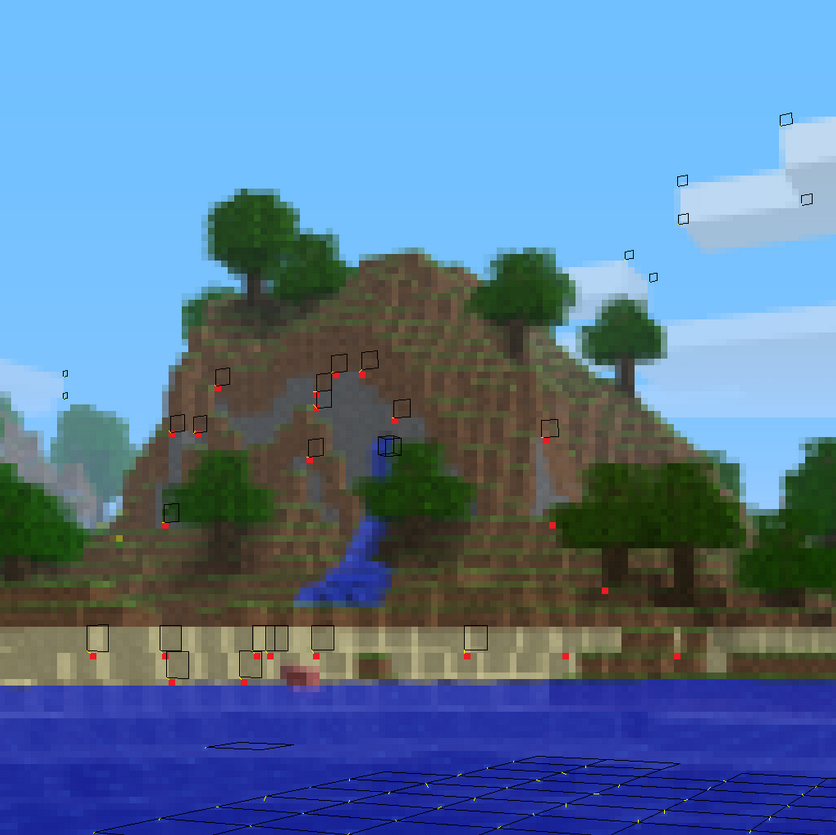
\includegraphics[width=\linewidth]{pfold.png}
\end{center}

Были получены оценки, которые позже были улучшены с помощью большего числа точек с изображения.  
Итоговыми оценками стали:
После небольшого визуального изменения параметров был найден окончательный, очень точный набор координат:
\begin{enumerate}
    \item Игрок смещен относительно водопада на (x = -66,84, y = -10,38, z = 31,72).
    \item Тангаж -8,297, рыскание -119,23.
    \item Глобальная координата z: z = -31 (в зависимости от положения облака).
    \item Разрешение экрана — 1600x1116, исходное кадрирование начинается с пикселя (622, 284) (полное кадрирование — 512x512). % Added comma for better readability
\end{enumerate}

Это было очень важное событие, поскольку оно дало координату Z водопада.

\subsection{Статистический подход}

Толщина земли в каждой точке определяется шумом Перлина, который зависит от сида в комбинации со случайными "аномалиями", которые одинаковы для всех сидов.  
Используя статистические методы (не удалось найти точное описание), была получена координата X = 116.  

Таким образом были получены точные координаты (116, 76, -31).

\subsection{Поиск сида}

Был написан алгоритм на Cuda, который по паттернам земли и песка отбрасывал большинство сидов. Для распределения перебора всех $2^{48}$ уникальных сидов была использована платформа BOINC.  
Спустя месяцы поиска алгоритм отсеял все сиды, кроме 700'000, совпадающих по паттернам. Для их проверки был использован более точный алгоритм, который обнаружил следующий сид: 3257840388504953787.  

\subsection{Результаты}

Весь процесс поиска занял порядка 8 месяцев и задействовал порядка 3 тысяч человек для брутфорса всех возможных сидов.\\ % Added period for sentence completion
В конечном итоге был найден сид, на котором был сделан снимок: 3257840388504953787.

\begin{center}
    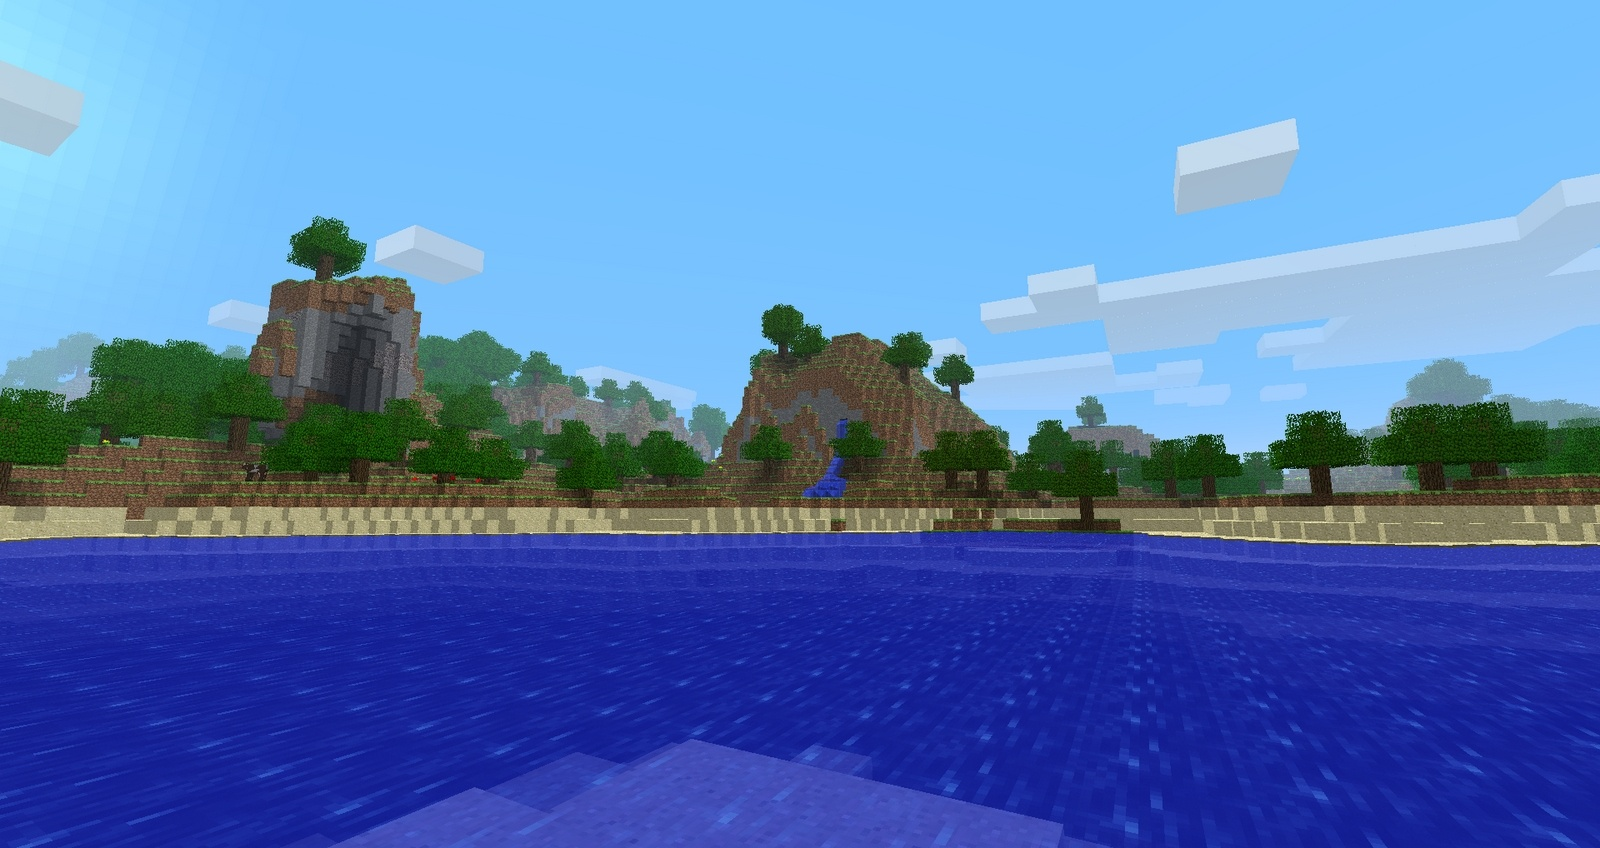
\includegraphics[width=\linewidth]{final.png}
\end{center}

% \subsection{Воссоздание ландшафта}

% Было предпринято как минимум 2 крупные попытки воссоздания. Между этими двумя попытками


\section{Источники}
\begin{itemize}
    \item \href{https://packpng.com/}{\textbf{Pack.PNG - Проект}}
    \item \href{https://minecraftathome.com/projects/packpng.html}{\textbf{Pack.PNG - Minecraft@Home}}
    \item \href{https://www.youtube.com/watch?v=ea6py9q46QU}{\textbf{Pack.PNG has been FOUND! - Here's how they did it}}
\end{itemize}

\end{document}
